\begin{figure}[H]
    \centering
    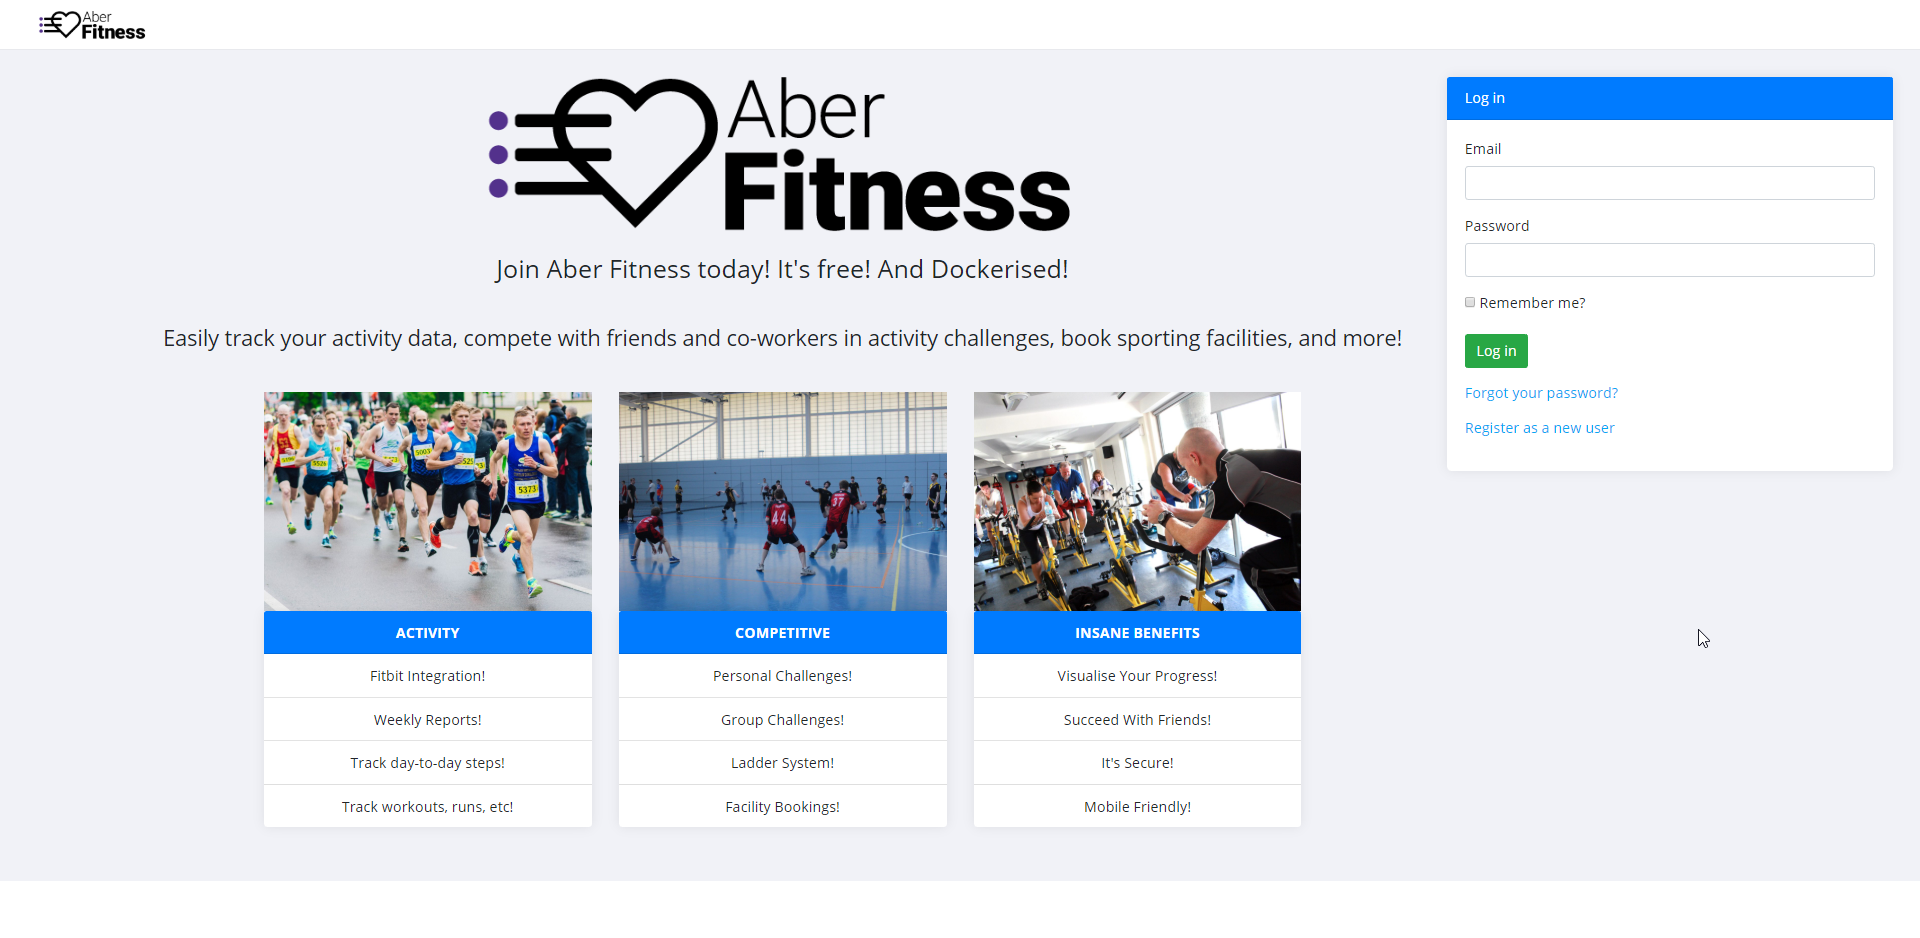
\includegraphics[width=\textwidth]{Images/service_landing_page.png}
    \caption{Gatekeeper is responsible for serving up the landing page, which features a user log in form and the ability for users to register to join Aber Fitness}
\end{figure}

During the analysis and planning stages it quickly became apparent that a central authentication and authorization system would be required. The Gatekeeper service is responsible for providing this, and does so by acting as both an OAuth 2.0 Authorization Server, and an OpenID Connect Identity Provider (IDP). Such a set up provides a number of benefits, including seamless Single Sign-On (SSO), relative ease of implementation due to the abundance of available libraries, separation of concerns by decoupling authentication \& authorization from each microservice, and the theoretical ability to allow third-party access to Aber Fitness APIs in the future.

\subsubsection{IdentityServer4}

Rather than attempting to implement our own OAuth 2.0 server, it seemed beneficial in terms of both security and development time to use an existing solution. After thorough investigation of the available implementations, IdentityServer4\cite{identityserver4} was chosen as it not only fully implements the specification of OAuth 2.0 and OpenID Connect, but is also certified by the OpenID Foundation, and is part of the .NET Foundation\cite{identityserver4docs}. Thorough documentation is available, the project is open-source with a permissive license, and the library is specifically designed for .NET Core 2.

\subsubsection{OAuth Overview}

Two basic OAuth 2.0 flows are used within Aber Fitness - Authorization Code (including the hybrid flow OpenID Connect extension) for applications with a GUI wishing to identify users, and Client Credentials for API authorization between the various microservices.

When a user first attempts to access a service where authentication is required, they are redirected to Gatekeeper in order to log in. Once logged in, they are redirected back to the client application which completes a token validation process in order to verify the login. To facilitate SSO, users which are already logged in to Gatekeeper will be seamlessly redirected back to the client application with no action required from them.

\begin{figure}[H]
    \centering
    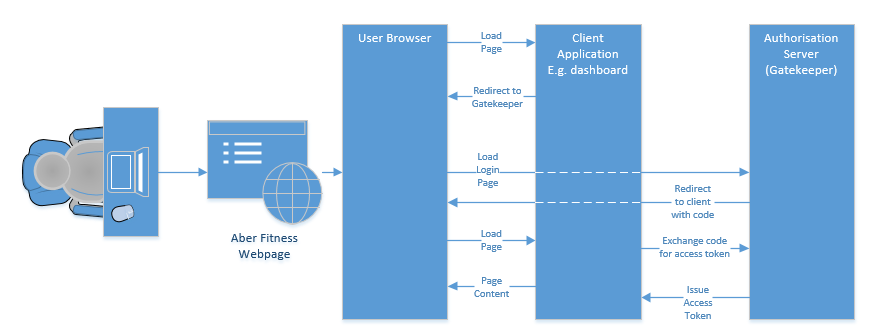
\includegraphics[width=\textwidth]{Images/gatekeeper_authcode_flow.png}
    \caption{Simplified diagram showing overview of the OAuth 2.0 Authorization Code flow.}
\end{figure}

On subsequent requests, a redirect to Gatekeeper is not usually required. Access tokens are valid for one hour, with the client being able to obtain new tokens via the use of a refresh token. Redirection to Gatekeeper should only be required if the user has cleared their browser cookies, or those cookies have become invalidated for some reason.

When a microservice wishes to call the API of another microservice, they obtain a client credentials access token from Gatekeeper, and send it in the Authorization header of the request they are making. Access tokens have a limited number of scopes (services) for which they are valid, and the service receiving the request will reject the token should it not contain the scope required for that service. Once the content of access token has been checked, the signature of the token is validated using the JSON Web Key Set (JWKS) available from Gatekeeper. This is essentially a public key which can be used to verify that the access token was indeed issued by Gatekeeper.

\begin{figure}[H]
    \centering
    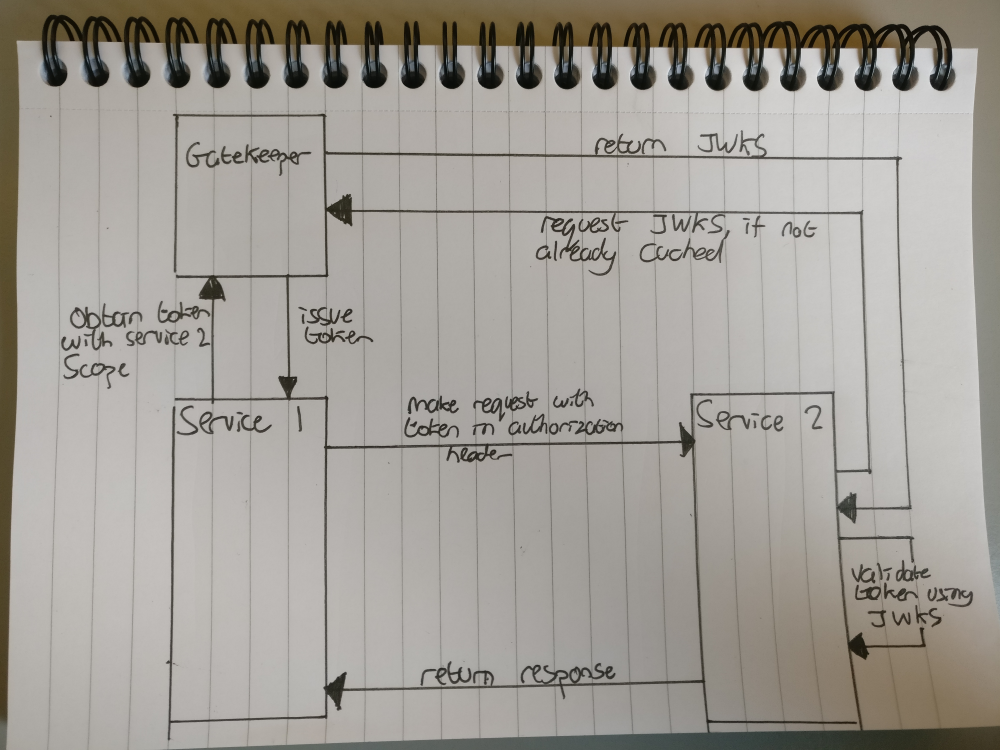
\includegraphics[width=0.7\textwidth]{Images/gatekeeper_clientcredentials_flow.png}
    \caption{Simplified diagram showing overview of the OAuth 2.0 Client Credentials flow.}
\end{figure}

There was some consideration as to whether client credentials was the correct flow to use for authorization when obtaining user resources within Aber Fitness. Typically you would require an access token specific to that user, obtained using the authorization code flow, in order to access resources such as activity data belonging to that user. Eventually it was decided that the authorization code flow would be more relevant to third-party applications wishing to access our APIs. As all microservices within Aber Fitness can be considered as belonging to the same overall system, it seemed that the client credentials flow was sufficient to authorize access to data from other services within the Aber Fitness system.

\subsubsection{Implementation Details}

Clients built using .NET core were provided with written documentation on how to use the client libraries provided by IdentityServer4 (another benefit of using this solution), and after some minor initial configuration, enabling authentication and authorization within their application was as simple as adding an attribute to their controller. Clients built using Java were not able to use libraries provided by IdentityServer4, but were instead able to take advantage of existing OAuth 2.0 client libraries available for that language.

One important consideration for Gatekeeper was the proper management of .NET Core data protection keys. Mishandling of these keys would cause every user session and access token within the system to become invalidated every time the application was relaunched, as the combination of the ephemeral nature of Docker containers, and the default behaviour of .NET Core would cause the keys to be re-generated on each launch. The solution was to require that the application be provided with a path to a folder, via environment variable, to which it could persist data protection keys across launches. In practise, this meant a Docker volume was mounted on the container running Gatekeeper, and the application could continue using the same keys regardless of updates to the Docker image or container restarts.

Unfortunately, as the OAuth 2.0 administration pages for Gatekeeper were being implemented, it was found that access to the underlying IdentityServer4 entities via Entity Framework was not as simple as previously thought. Whilst top-level models could be retrieved from the database using the contexts provided by IdentityServer4, there was seemingly no access to the underlying child objects. The database schema provided by IdentityServer4 seemed unnecessarily complex in some areas, possibly even a purposeful design choice in order to encourage users to purchase a licence for their commercial management software\cite{identityserver4adminui}. Due to this complexity, we only implemented functionality to create and delete OAuth 2.0 resources, without the ability to edit them. Whilst somewhat inconvenient, this was deemed sufficient for the needs of this project as these resources would rarely need editing anyway.

\subsubsection{Alternatives}

A number of alternatives were considered, including OpenIddict\cite{openiddict} for .NET Core, and Connect2Id\cite{connect2id} for Java, however none of the alternatives investigated provided the same level of documentation and community support as IdentityServer4.

Additionally, alternative standards such as Security Assertion Markup Language (SAML) were investigated as an alternative to OAuth, and whilst SAML may have also provided all the necessary functionality, it was ultimately discarded as a choice due to the Aber Fitness developers being more familiar with OAuth 2.0, and for the avoidance of introducing XML data exchange between our services.
